\documentclass[final,hyperref={pdfpagelabels=false}]{beamer}

\usepackage[orientation=portrait,size=a0,scale=1.4]{beamerposter}

\usetheme{I6pd2}
\usepackage{xcolor}
\usepackage{caption}
\usepackage{amssymb}
\usepackage{amsmath}
\usepackage{amsfonts}
\usepackage{booktabs}
\usepackage{tcolorbox}
\graphicspath{{Images/}}
\usepackage[english]{babel}
\usepackage[tight,footnotesize]{subfigure}
\usepackage{amsmath,amsthm,amssymb,latexsym}

\usepackage{tikz}
\usetikzlibrary{arrows,shapes,backgrounds,shapes.misc,fit,bayesnet}

\setbeamerfont{footnote}{size=\tiny}

\definecolor{Blue}{HTML}{000080}

\usecaptiontemplate{\small\structure{\insertcaptionname~\insertcaptionnumber: }\insertcaption}

\title{Bayesian Nonparametric Motor-skill Representations \\ for Efficient Learning of Robotic Clothing Assistance}
\author{Nishanth Koganti$^{1,2}$, Tomoya Tamei$^1$, Kazushi Ikeda$^1$, Tomohiro Shibata$^2$}
\institute{$^1$Nara Institute of Science and Technology, Japan~~$^2$Kyushu Institute of Technology, Japan}

\newcommand{\leftfoot}{Neural Information Processing Systems 2016}
\newcommand{\rightfoot}{Workshop on Practical Bayesian Nonparametrics}

\begin{document}

\addtobeamertemplate{block end}{}{\vspace*{0.5ex}}
\addtobeamertemplate{block alerted end}{}{\vspace*{2ex}}

\begin{frame}[t]

\begin{columns}[t]
  \begin{column}{.02\linewidth}\end{column}

  \begin{column}{0.47\linewidth}
    \begin{block}{Introduction}
      \begin{center}
        \textbf{Objective}: Motor-skill learning for complex robotic tasks is challenging due to high task variability. Robotic clothing assistance is one problem that can improve the quality-of-life for elderly and disabled. In this study, we propose a representation to encode task specific motor-skills using Bayesian nonparametric latent space learning and rely on this for data-efficient reinforcement learning.
      \end{center}

      \begin{columns}[t]
        \begin{column}{0.6\linewidth}
          \vskip0.5em
          Tamei et. al. \footnotemark[1] developed clothing assistance framework for dual-arm robots:\vskip0.5em
          \begin{itemize}
            \item \textbf{Reinforcement Learning} to acquire motor skills.
            \item Policy representation inefficient for generalization.
          \end{itemize}

          \begin{figure}
            \centering
            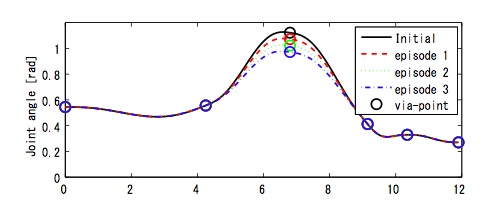
\includegraphics[height=0.06\textheight, width=0.8\textwidth]{policy.png}
          \end{figure}
        \end{column}

        \begin{column}{0.4\linewidth}
          \begin{figure}
            \centering
            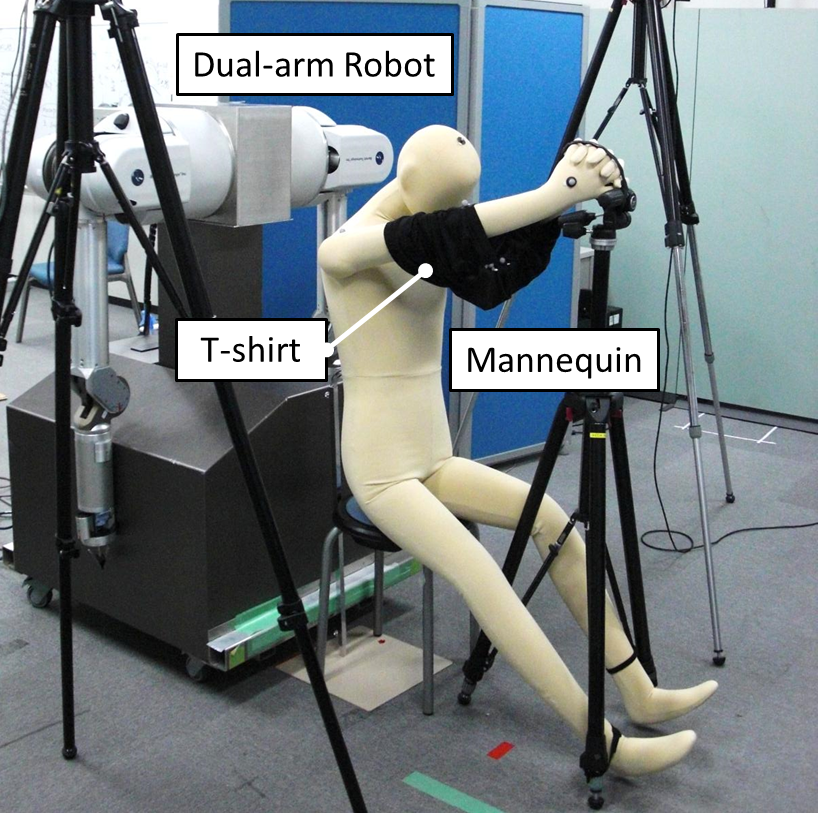
\includegraphics[width=0.9\textwidth]{setup.png}
          \end{figure}
        \end{column}
      \end{columns}
    \end{block}
  \end{column}

  \begin{column}{0.47\linewidth}
    \begin{block}{Latent Space Reinforcement Learning}
      \begin{columns}[t]
        \begin{column}{0.65\textwidth}
          Combine Reinforcement Learning (RL) with Dimensionality Reduction (DR):
          \begin{itemize}
            \item Tractable search space reduces learning time.
            \item Latent space can model task space constraints.
          \end{itemize}
        \end{column}

        \begin{column}{0.35\textwidth}
          \vskip-2em
          \begin{figure}
            \centering
            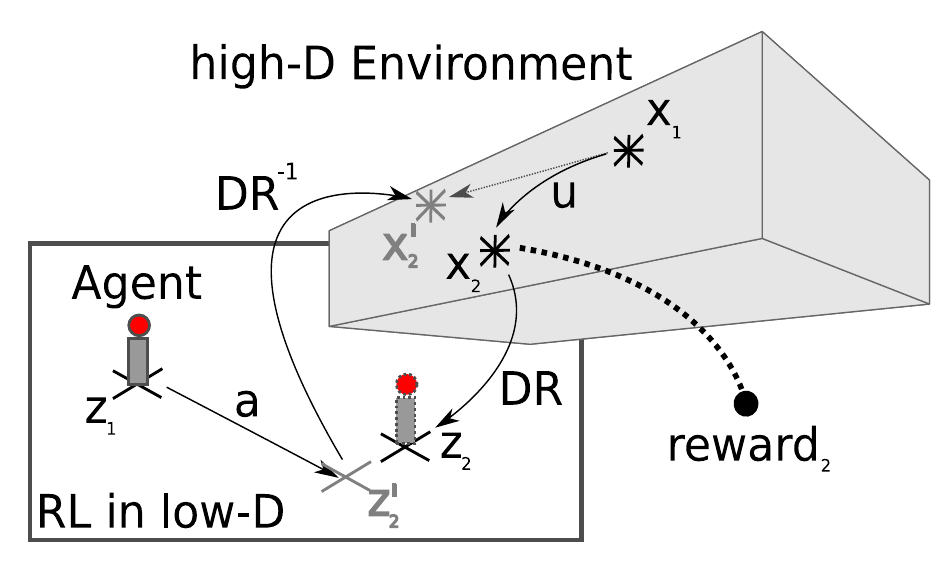
\includegraphics[width=0.8\textwidth]{latentrl.png}
            \caption*{\footnotesize{Bitzer et al., 2010 \footnotemark[2]}}
          \end{figure}
        \end{column}
      \end{columns}

      \begin{columns}[t]
        \begin{column}{0.3\textwidth}
          \vskip-1em
          \begin{figure}
            \centering
            \caption*{Bitzer et al., 2010 \footnotemark[2]}
            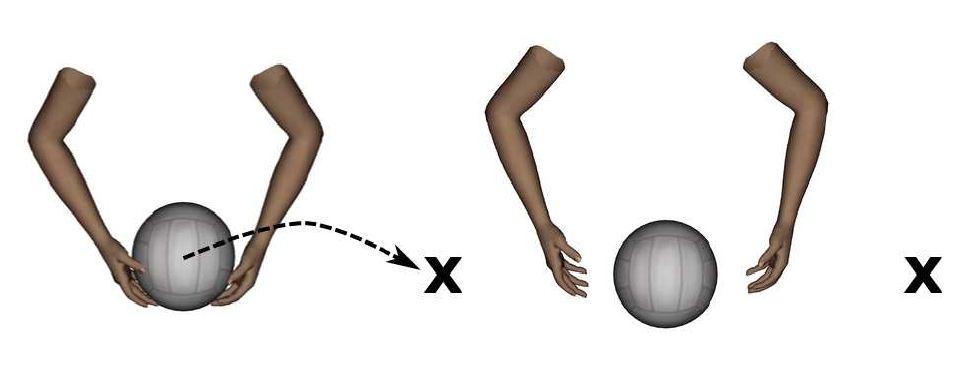
\includegraphics[width=0.8\textwidth]{bitzer.png}
          \end{figure}

          \begin{figure}
            \centering
            \caption*{Luck et al., 2014 \footnotemark[3]}
            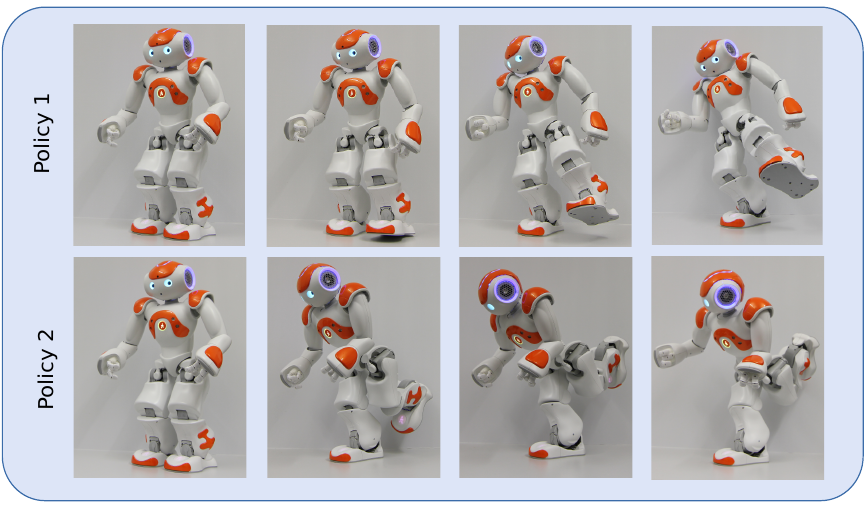
\includegraphics[width=0.8\textwidth]{luck.png}
          \end{figure}
        \end{column}

        \begin{column}{0.6\textwidth}
          \vskip0.5em
          Existing frameworks have limitations:\vskip0.5em
          \begin{itemize}
            \item \textbf{Bitzer et al., 2010 \footnotemark[2]}: DR as preprocessing before RL
              \begin{itemize}
                \item MAP estimate of latent space leads to overfitting.\\~\\
              \end{itemize}
              \item \textbf{Luck et al., 2014 \footnotemark[3]}: Combine DR and RL under EM-formulation
                \begin{itemize}
                  \item Linear model used for DR can be insufficient for complex tasks.
                \end{itemize}
          \end{itemize}
        \end{column}
      \end{columns}
    \end{block}
  \end{column}

  \begin{column}{.02\linewidth}\end{column}
\end{columns}

\begin{columns}[t]
  \begin{column}{0.02\linewidth}\end{column}

  \begin{column}{0.96\linewidth}
    \begin{block}{Proposed Method}
      \begin{columns}[t]
        \begin{column}{0.33\linewidth}
          \centering \large \textbf{Bayesian Gaussian Process LVM}

          \begin{columns}
            \begin{column}{0.8\textwidth}
              \begin{itemize}
                \item Latent variable model (Titsias et al., 2010 \footnotemark[4]):
                  \begin{equation*}
                    \mathbf{y} = f(\mathbf{x}) + \epsilon,~~\epsilon \in \mathcal{N}(\mathbf{0}, \sigma^2 \mathbf{I})
                  \end{equation*}
                  \begin{itemize}
                    \item $\mathbf{y} \in \mathbb{R}^D$: Observed Variable
                    \item $\mathbf{x} \in \mathbb{R}^Q (Q \ll D)$: Unknown latent variable
                    \item $f: \mathbf{x} \rightarrow \mathbf{y}$: Gaussian Process mapping
                  \end{itemize}
              \end{itemize}
            \end{column}
            \begin{column}{0.2\textwidth}
              \begin{figure}
                \centering
                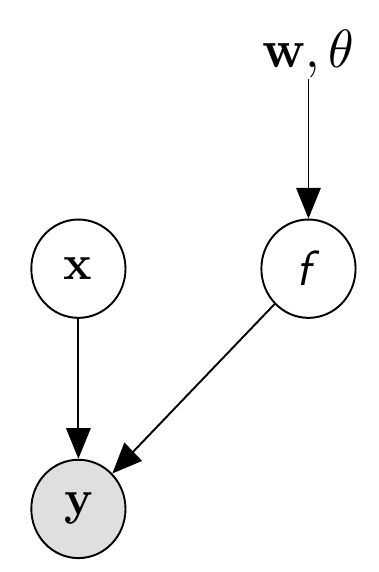
\includegraphics[width=\textwidth]{lvm.png}
              \end{figure}
            \end{column}
          \end{columns}
          \begin{figure}
            \centering
            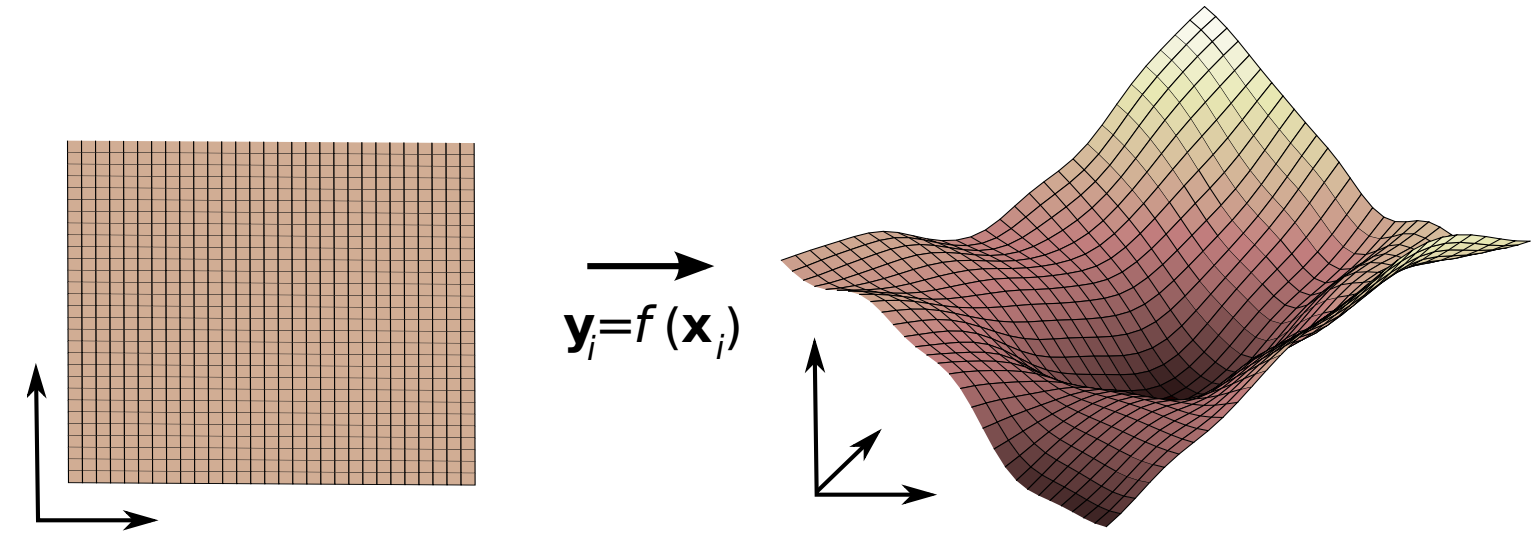
\includegraphics[width=0.8\textwidth]{nonlinearMap.png}
          \end{figure}

          \begin{itemize}
            \item \textbf{Bayesian Inference}: Posterior distribution on the latent space.
              \begin{equation*}
                p(\mathbf{Y}) = \int_{\mathbf{X}} p(\mathbf{Y}|\mathbf{X}) p(\mathbf{X}) d\mathbf{X}
              \end{equation*}
            \item Automatic dimensionality reduction possible using ARD kernel \footnotemark[5]:
                \begin{equation*}
                  k(x,x') = \sigma_f^2 \exp \left( - \frac{1}{2} \Sigma_{q=1}^Q \mathbf{w_q} (x_q - x_q')^2 \right)
                \end{equation*}
          \end{itemize}
        \end{column}

        \begin{column}{0.34\linewidth}
          \centering \large \textbf{Motor-skills in Latent Space}
          \begin{tcolorbox}[width=0.9\textwidth, colback=red!75!white, colframe=red!5!white]
            \small \centering \textcolor{white}{\textbf{Problem}: Design of robust motor-skills framework is crucial for real-world implementation on low-cost robots.}
          \end{tcolorbox}

          \begin{tcolorbox}[width=0.9\textwidth, colback=blue!75!white, colframe=blue!5!white]
            \small \centering \textcolor{white}{\textbf{Solution}: Use Bayesian nonparametric dimensionality reduction for efficient learning of clothing skills.}
          \end{tcolorbox}
          \vskip0.5em
          \begin{figure}
            \centering
            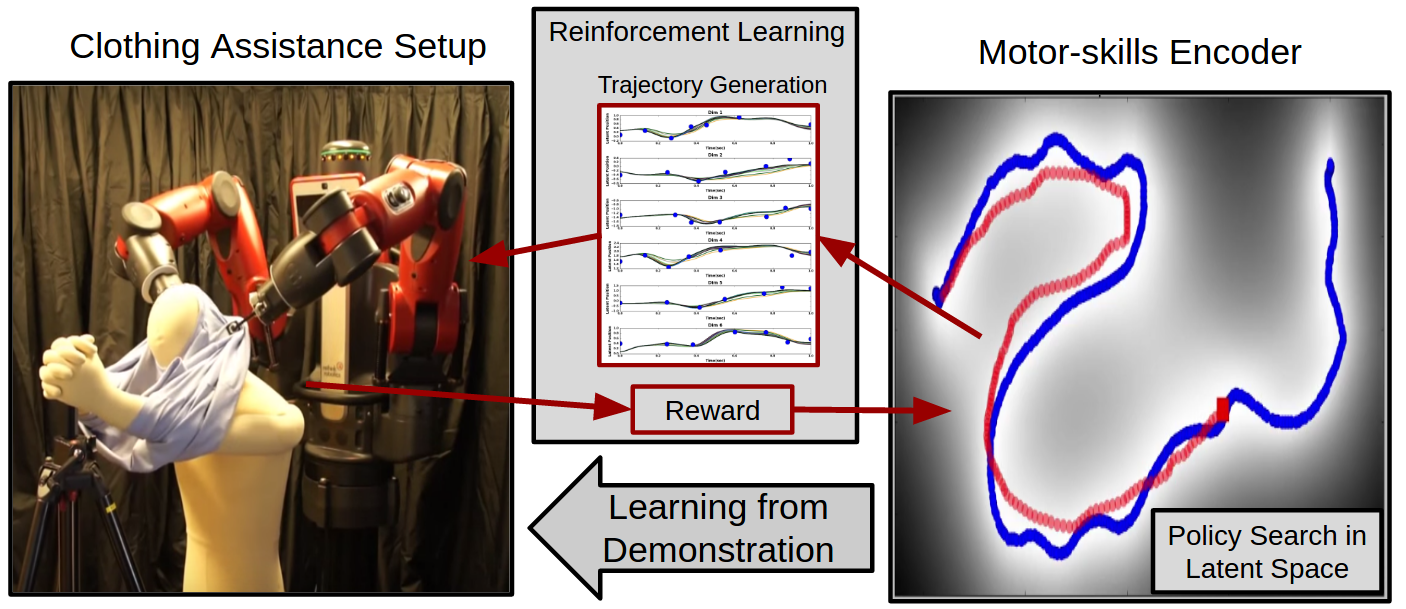
\includegraphics[width=\textwidth]{overview.png}
          \end{figure}

          \begin{itemize}
            \item \small \textbf{Learning from Demonstration}: BGPLVM latent space as user-friendly controller for kinesthetic demonstration.
            \item \small \textbf{Reinforcement Learning}: Apply reinforcement learning with BGPLVM latent space as action space.
          \end{itemize}
        \end{column}

        \begin{column}{0.33\linewidth}
          \centering \large \textbf{Reinforcement Learning Formulation}

          \begin{itemize}
            \item Cross Entropy Method (CEM)\footnotemark[6] for policy improvement:
              \begin{equation*}
                \begin{array}{c}
                  \theta^* \sim \mathcal{N} (\theta | \mathbf{\mu}^*, \Sigma^{*})\\
                  \mathbf{\mu}^* := \text{mean}(\text{argmax}~ \theta_{\text{old}}),~~\Sigma^{*} := \text{var}(\text{argmax} ~\theta_{\text{old}})
                \end{array}
              \end{equation*}
            \item \textbf{Policy representation}: Dynamic Movement Primitives (DMP) \footnotemark[7]:
              \begin{equation*}
                \begin{array}{c}
                  \tau \ddot{x} = K(g-x) -D\dot{x} + (g - x_0)f\\
                  \displaystyle f(s) = \frac{\Sigma_i w_i \psi_i(s)s}{\Sigma_i \psi_i(s)}, \text{ where } \tau \dot{s} = - \alpha s
                \end{array}
              \end{equation*}
            \item \textbf{Reward function}: Distance from desired Via-points to current policy:
              \begin{equation*}
                R(\pi(\theta)) = \Sigma_{i = 1}^{n_{\text{dims}}} \Sigma_{j = 1}^{n_{\text{via}}} \| V_{i,j} - \pi_i(\theta, t_{i,j}) \|^2
              \end{equation*}
          \end{itemize}

          \begin{figure}
            \centering
            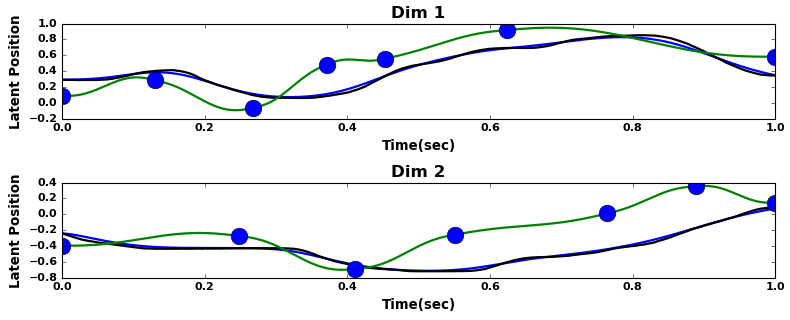
\includegraphics[width=0.8\textwidth]{trajectory.png}
          \end{figure}
        \end{column}
      \end{columns}
    \end{block}
  \end{column}

  \begin{column}{0.02\linewidth}\end{column}
\end{columns}

\begin{block}{Experimental Results}

  \begin{columns}[t]
    \begin{column}{0.02\linewidth}\end{column}

    \begin{column}{0.4\linewidth}
      \centering \textbf{\large Generalization in Latent Space}\\

      \begin{columns}
        \begin{column}{0.5\textwidth}
          \begin{figure}
            \centering
            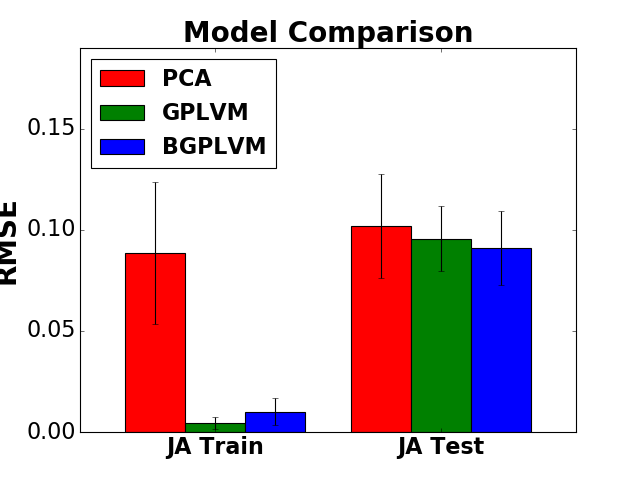
\includegraphics[width=0.9\textwidth]{jaError.png}
          \end{figure}
        \end{column}
        \begin{column}{0.5\textwidth}
          \centering \textbf{Evaluation}: Reconstruction error of latent space with RMS Error \footnotemark[1]. \\
          \vskip1em
          \textbf{Dataset}: Clothing trajectories for 4 postures: Shoulder Angle $\in \{65^o,70^o,75^o,80^o\}$.
        \end{column}
      \end{columns}
      \vskip1em
      \begin{columns}
        \begin{column}{0.36\textwidth}
          \centering \textbf{PCA}
          \vskip-0.5em
          \begin{figure}
            \centering
            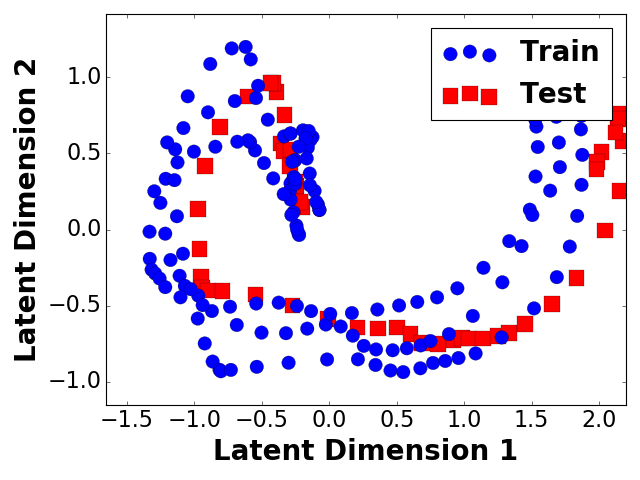
\includegraphics[width=\textwidth]{jaPCA.png}
          \end{figure}
        \end{column}
        \begin{column}{0.36\textwidth}
          \centering \textbf{GPLVM}
          \vskip-0.5em
          \begin{figure}
            \centering
            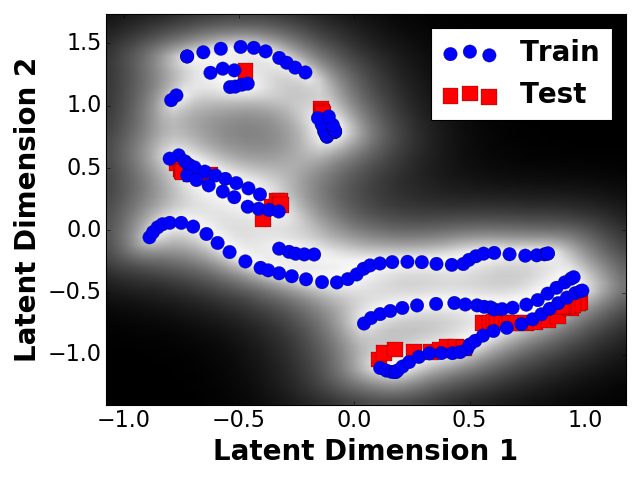
\includegraphics[width=\textwidth]{jaGPLVM.png}
          \end{figure}
        \end{column}
        \begin{column}{0.36\textwidth}
          \centering \textbf{BGPLVM}
          \vskip-0.5em
          \begin{figure}
            \centering
            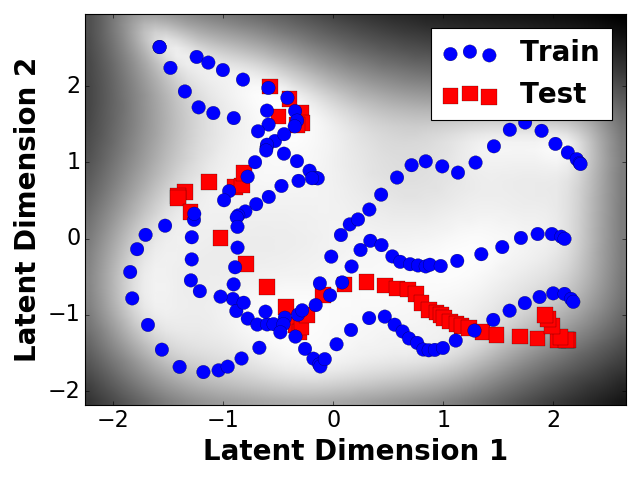
\includegraphics[width=\textwidth]{jaBGPLVM.png}
          \end{figure}
        \end{column}
      \end{columns}
    \end{column}

    \begin{column}{0.05\linewidth}\end{column}

    \begin{column}{0.4\linewidth}
      \centering \large \textbf{Effectivity of Search Space}\\

      \begin{center}
        Apply Reinforcement Learning in different action spaces with same formulation:
      \end{center}

      \begin{itemize}
        \item Parameters: $50 \times n_{\text{dims}}$ basis functions in DMP.
        \item Cross Entropy Method: 50 rollouts per iteration.
        \item Policy Update: 5 best rollouts per iteration
      \end{itemize}
      \vskip-2em
      \begin{columns}[t]
        \begin{column}{0.35\textwidth}
          \vskip2em
          \begin{itemize}
            \item BGPLVM search space performs best as it uses non-linear mapping and avoids overfitting. \vskip1em
            \item PCA performs better than GPLVM as MAP estimation of GPLVM overfits to training data.
          \end{itemize}
        \end{column}
        \begin{column}{0.65\textwidth}
          \begin{figure}
            \centering
            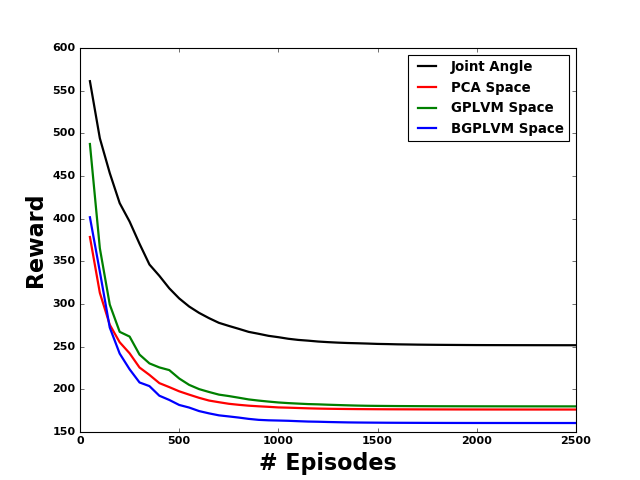
\includegraphics[width=\textwidth]{rlcurve.png}
          \end{figure}
        \end{column}
      \end{columns}
    \end{column}

    \begin{column}{0.02\linewidth}\end{column}
  \end{columns}
\end{block}

\begin{columns}[t]

  \begin{column}{.02\textwidth}\end{column}

  \begin{column}{0.47\textwidth}
    \begin{block}{Future Work}
      \begin{itemize}
        \item \textbf{Immediate Goal}: BGPLVM for learning clothing assistance skills:
          \begin{itemize}
            \item Use robot proprioceptive and depth sensor readings as state representation.
            \item Incorporate dynamics prior and task-specific covariance functions.
          \end{itemize}
          \vskip0.5em
        \item \textbf{Long Term Goal}: Combine policy search RL and BGPLVM:
          \begin{itemize}
            \item EM-formulation with BGPLVM parameters as latent variables.
            \item Modify variational inference framework for RL setting.
          \end{itemize}
        \end{itemize}
    \end{block}
  \end{column}

  \begin{column}{0.47\textwidth}
    \begin{block}{References}
      \nocite{*}
      \scriptsize{
      \bibliographystyle{unsrt}

      \begin{thebibliography}{10}
        \bibitem{tamei}
        Tamei, T. et al., ``Reinforcement learning of clothing assistance'', in \emph{IEEE-RAS Humanoids 2011}

        \bibitem{bitzer}
        Bitzer, S. et al., ``Using dimensionality reduction in reinforcement learning'' in \emph{IEEE/RSJ IROS, 2010}

        \bibitem{luck}
        Luck, K. S. et al., ``Latent space policy search for robotics'' in \emph{IEEE/RSJ IROS, 2014}

        \bibitem{bgplvm}
        Titsias, M. K. et al., ``Bayesian Gaussian Process Latent Variable Model'', in \emph{AISTATS 2011}

        \bibitem{gp}
        Williams, C. et al., ``Gaussian processes for machine learning'' by \emph{MIT Press 2006}.

        \bibitem{cem}
        De Boer, P. et al., ``A tutorial on the cross-entropy method'' in \emph{Annals of operations research 2005}.

        \bibitem{dmp}
        Ijspeert, A. J. et al., ``Dynamical movement primitives: learning attractor models for motor behaviors'', in \emph{Neural computation 2013}.
      \end{thebibliography}}
    \end{block}
  \end{column}

  \begin{column}{.02\textwidth}\end{column}
\end{columns}

\end{frame}

\end{document}
